
\chapter{Methodology}

This chapter presents the approach used for this research.
 Fig. \ref{phd-methodology} summarizes the steps.

\begin{figure}[h]
\centering
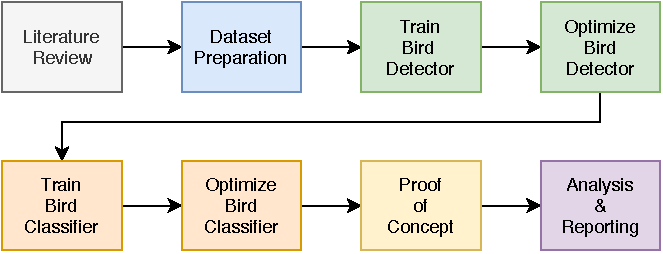
\includegraphics[width=.8\textwidth]{phd-methodology}
\caption{Research methodology.}
\label{phd-methodology}
\end{figure}

The steps are:
\begin{enumerate}
    \item \textbf{Literature review}: find an interesting research topic and gaps to explore. This stage has been completed and documented in Chapter 2.
    \item \textbf{Dataset preparation}: downloading sound files from open data sources and generate sufficient samples for CNN training
    \item \textbf{Bird detector design}: explore configurations of binarized neural network to detect bird vocalizations
    \item \textbf{Bird classifier design}: explore configurations of convolutional neural network to detect up to 20 different species
    \item \textbf{Proof-of-concept}: implement the cascade classifer on a suitable edge platform
    \item \textbf{Analysis and reporting}: wrap-up of the project
\end{enumerate}

\section{Dataset Preparation}

Unlike other machine learning datasets, most sound datasets are cannot be directly used training a CNN. This is because sound files vary in length, quality, and annotations.
The result of the dataset preparation stage is a collection of audio files, each of length 1 second containing a specific sound sometime in the file.

All sound files are be resampled to 8 kHz. According to the Nyquist theorem, the highest frequency in a sample is half the sampling frequency. At the chosen sampling frequency, sounds 4 kHz and below are preserved. The maximum of 4 kHz is sufficient to cover the frequency range of bird vocalizations.

Two datasets will be required. The first dataset is used to train the bird detector. The dataset should contain negative samples or non-bird sounds as well as many variations of bird sounds. Table \ref{serdb} lists sources of sounds for this dataset. Twenty thousand sound samples are to be collected for this dataset. The majority of the 10,000 negative samples will come from the Urban8k which contain 10 urban sound classes: air\_conditioner, car\_horn, children\_playing, dog\_bark, drilling, engine\_idling, gun\_shot, jackhammer, siren, and street\_music. The remaining positive and negative samples are to be derived from the Warbler dataset.

\begin{table}[h]
    \centering
    \small
    \caption{Environmental sound databases some of which contain bird sounds.}
    \label{serdb}
	\begin{tabular}{p{1in}p{4.5in}}
	\toprule
	\textbf{Dataset} & \textbf{Contents} \\
	\midrule
	Freesound & More than 400,000 crowdsourced sounds \\
	freefield1010 & >7,000 excerpts from field recordings around the world, derived from FreeSound  \\
	Urban8k & 8732 labeled sound excerpts (<=4s) of urban sounds from 10 classes, derived from Freesound \\
	ESC-50  & 2000 environmental recordings (50 classes, 40 clips per class) \\
    Warblr & 10,000 ten-second smartphone audio recordings from around the UK. Contains weather noise, traffic noise, human in addition to birds \\
    Chernobyl & >10,000 hours of audio recorded by unattended remote monitoring equipment in the Chernobyl Exclusion Zone (CEZ) \\
    \bottomrule
	\end{tabular}
\end{table}	

The second dataset contains  bird sounds labeled according to species. 
 Table \ref{birddb} lists sources of sounds for this dataset.
 From these sounds, 10,000 files for 10 species have already been collected.
 
\begin{table}[h]
    \centering
    \small
    \caption{Bird sound databases.}
    \label{birddb}
	\begin{tabular}{p{1.6in}p{3.9in}}
	\toprule
	\textbf{Dataset} & \textbf{Contents} \\
	\midrule
	Xeno-canto & >400,000 sound recordings,  >10,000 species worldwide \\
	Macaulay \mbox{Library} &  175,000 audio recordings covering 75 percent of the world's bird species \\
	British~\mbox{Birdsong} Dataset &  A subset of Xeno-canto: 264 recording of 88 UK birds\\
	NIPS4Bplus & 1867 files from 61 bird species recorded in France \\
	\bottomrule
	\end{tabular}
\end{table}	
	
 Fig. \ref{cascade-dataflow} summarizes the flow of data in the training process of both bird detector and bird identifier modules.


\begin{figure}%[H]
\centering
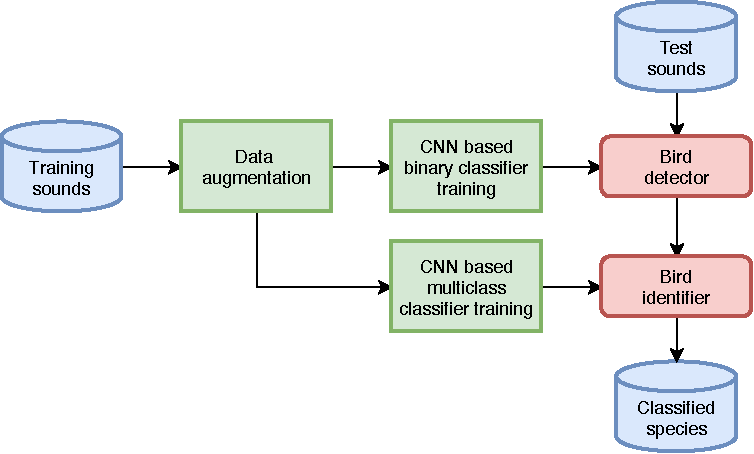
\includegraphics[width=.8\textwidth]{cascade-dataflow}
\caption{Data flow in proposed cascade bird classifier.}
\label{cascade-dataflow}
\end{figure}


\FloatBarrier

\section{Bird Detector}

The bird detector module is a binary classifier with a simple bird/no-bird output.
The module is intended to run continuously. Therefore, it must simple to reduce power consumption.
When this module detects a possible bird sound,  it passes the data to the bird species classifier.
This module can be considered a `weak' classifier. 
This module must be accurate enough so that it does not miss too many bird sounds.
At the same time, it is accept to have some false positives as these detections will nullified by the next module.

The proposed architecture is based on the binarized convolutional neural network (BNN)  \cite{Courbariaux2015,Simons2019}.
The topology for the BNN will follow the \textit{bulbul} CNN \cite{Grill2017}.
Each input sound file will be converted to a spectrogram.
The spectrogram image will be doubled in size and width before being binarized and used as input to the BNN.

Training of the detector will be done on a Ubuntu machine with 32 GB RAM and GeForce GTX 1080 Ti.
The software used is Keras and TensorFlow.

\section{Bird Classifier}

The bird classifier is small CNN with 20 outputs.
The number of outputs represent typical number birds around a housing area.
To compare power consumption with accuracy, the CNN will use 8-bit integer and 32-bit floating-point for weights and activations.
Several alternative configurations will be investigated to find tradeoffs in the design space.

The proposed training procedure is to use the spectrogram generated by the bird detector stage.
The spectrogram is altered before use by the CNN.
The result of the different features will be evaluated to find the highest score. Table \ref{variations} lists the proposed experiments.

\begin{table}[h]
    \caption{Variations in CNN design.}
    \label{variations}
    \centering\small
    \begin{tabular}{lll}
        \toprule
        \textbf{Topology} & \textbf{Parameters} & \textbf{Features} \\
        \midrule
        Variations in   & 8-bit integer & STFT \\
        layer count     & 32-bit FP     & Mel spectrogram \\
        \& types        &               & MFCC \\
                        &               & Cochleagram \\
        \bottomrule
    \end{tabular}
\end{table}

%\section{Proof of Concept}

To demonstrate the suitable of the best configuration of cascade classifier, the whole classifier is ported to Raspberry Pi. 

\section{Evaluation}

To evaluate the performance of each model, the following metrics are used.

\subsubsection{Precision}

This metric is defined as the proportion of true positives that are correctly identified by the detector. 
This metric is calculated by taking into account the True Positives (TP) and False Negatives (FN):

\[
\mathrm{Precision} = P = \frac{TP}{TP + FN}
\]

\subsubsection{Accuracy}

\[
\mathrm{Accuracy} = \frac{TP+TN}{\mathrm{total}}
\]

\noindent
Precision and accuracy are used on Keras code running on PC. The following metrics apply only classifier code runing on Raspberry Pi.

\subsubsection{Inferences-per-second (IPS)}}

The rate at which the bird classifier is capable of processing bird vocalizations

\subsubsection{Power consumption}

Power consumption is related to computational complexity.
For each investigated BNN/CNN pair, the number of MAC operations will be computed.
Then the power used will be checked using a power meter.
Lastly, the MAC versus power graph is derived.

\FloatBarrier

\section{Preliminary Results}

	\begin{itemize}
		\item For each long sound file
		\begin{itemize}
			\item find start and end points
			\item shift the sound pulse to beginning, middle and end
				to generate 3 sound files
		\end{itemize}
	\end{itemize}


\begin{figure}%[h]
    \centering
    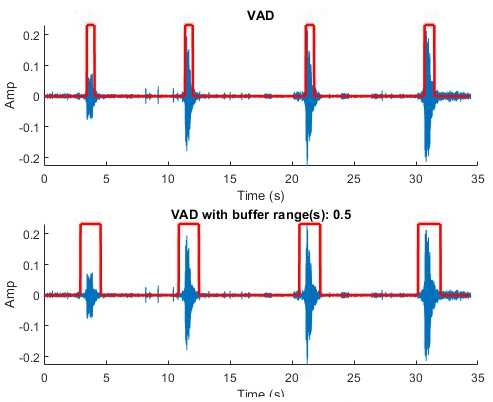
\includegraphics{aymen-audiosegment}
    \caption{Caption}
    \label{aymen-audiosegment}
\end{figure}

\begin{table}%[h]
	\caption{Species used in preliminary experiments.}
    \label{tab:my_label}
    \centering
	\begin{tabular}{clc}
    \toprule
	\textbf{Number} & 
	\textbf{Species} &
	\textbf{Soundfile count} \\
	\midrule
	1 & \textit{Mareca penelope} & 1000 \\
	2 & \textit{Turdus migratorius} & 1000 \\
	3 & \textit{Alaudala cheleensis} & 1000 \\
	4 & \textit{Cinnyris asiaticus} &  1000 \\
	5 & \textit{Zenaida asiatica} & 1000 \\
	6 & \textit{Lanius collurio} & 1000 \\
	7 & \textit{Icterus icterus} & 1000 \\
	8 & \textit{Glaucidium cuculoides} & 1000 \\
	9 & \textit{Columba oenas} & 1000 \\
	10 & \textit{Terpsiphone viridis} & 1000 \\	
	\bottomrule
	\end{tabular}
\end{table}

\begin{figure}%[h]
    \centering
    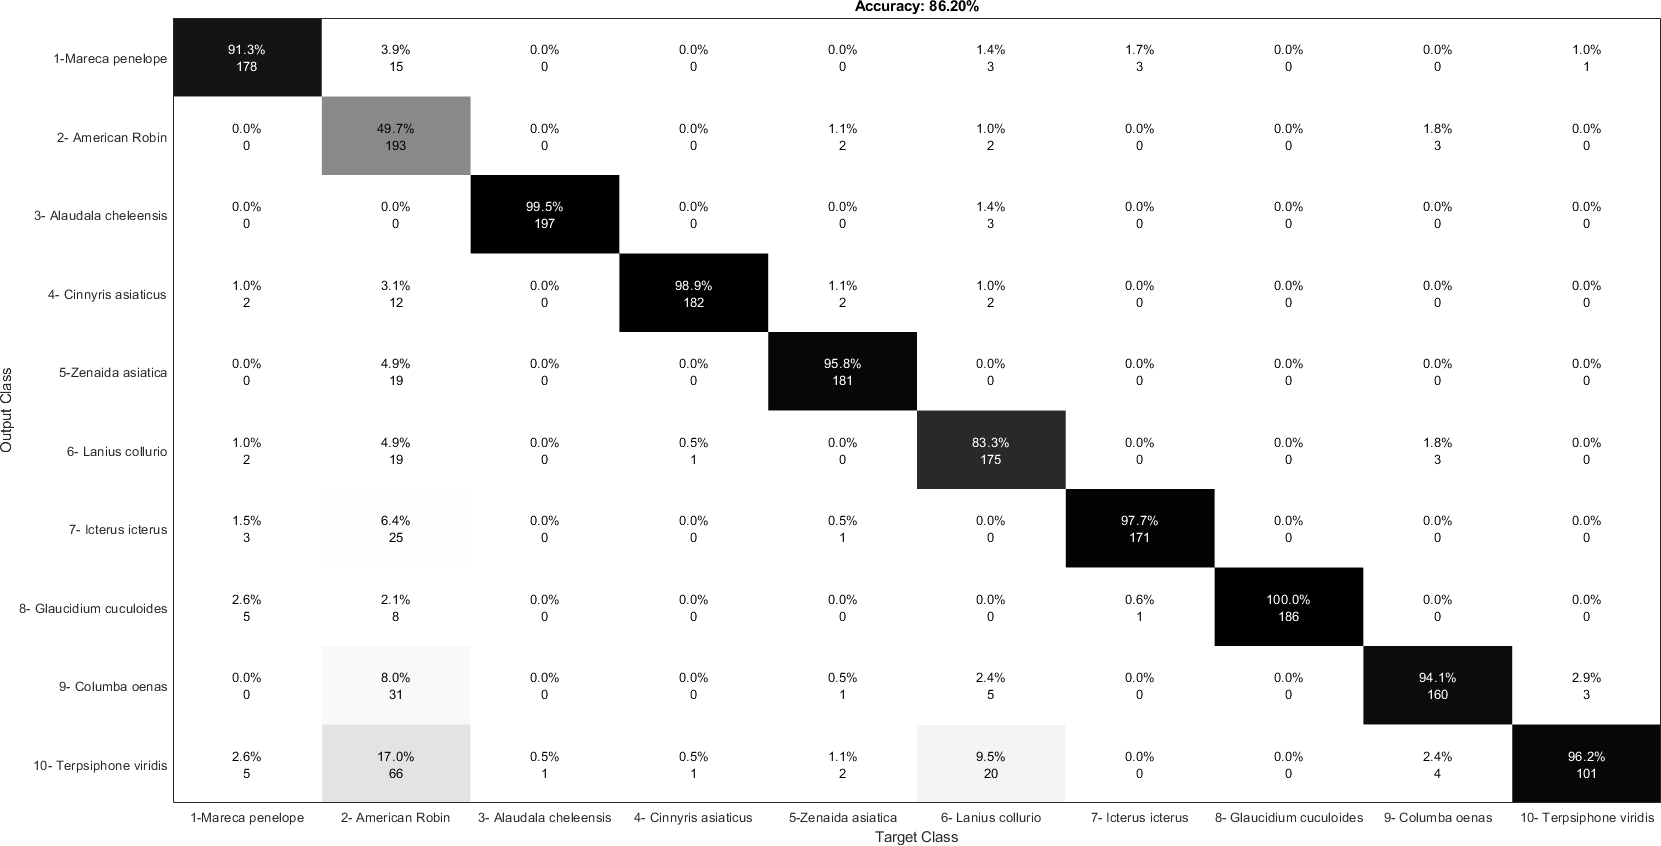
\includegraphics[width=\textwidth]{aymen-stft}
    \caption{STFT confusion matrix.}
    \label{aymen-stft}
\end{figure}

\begin{figure}%[h]
    \centering
    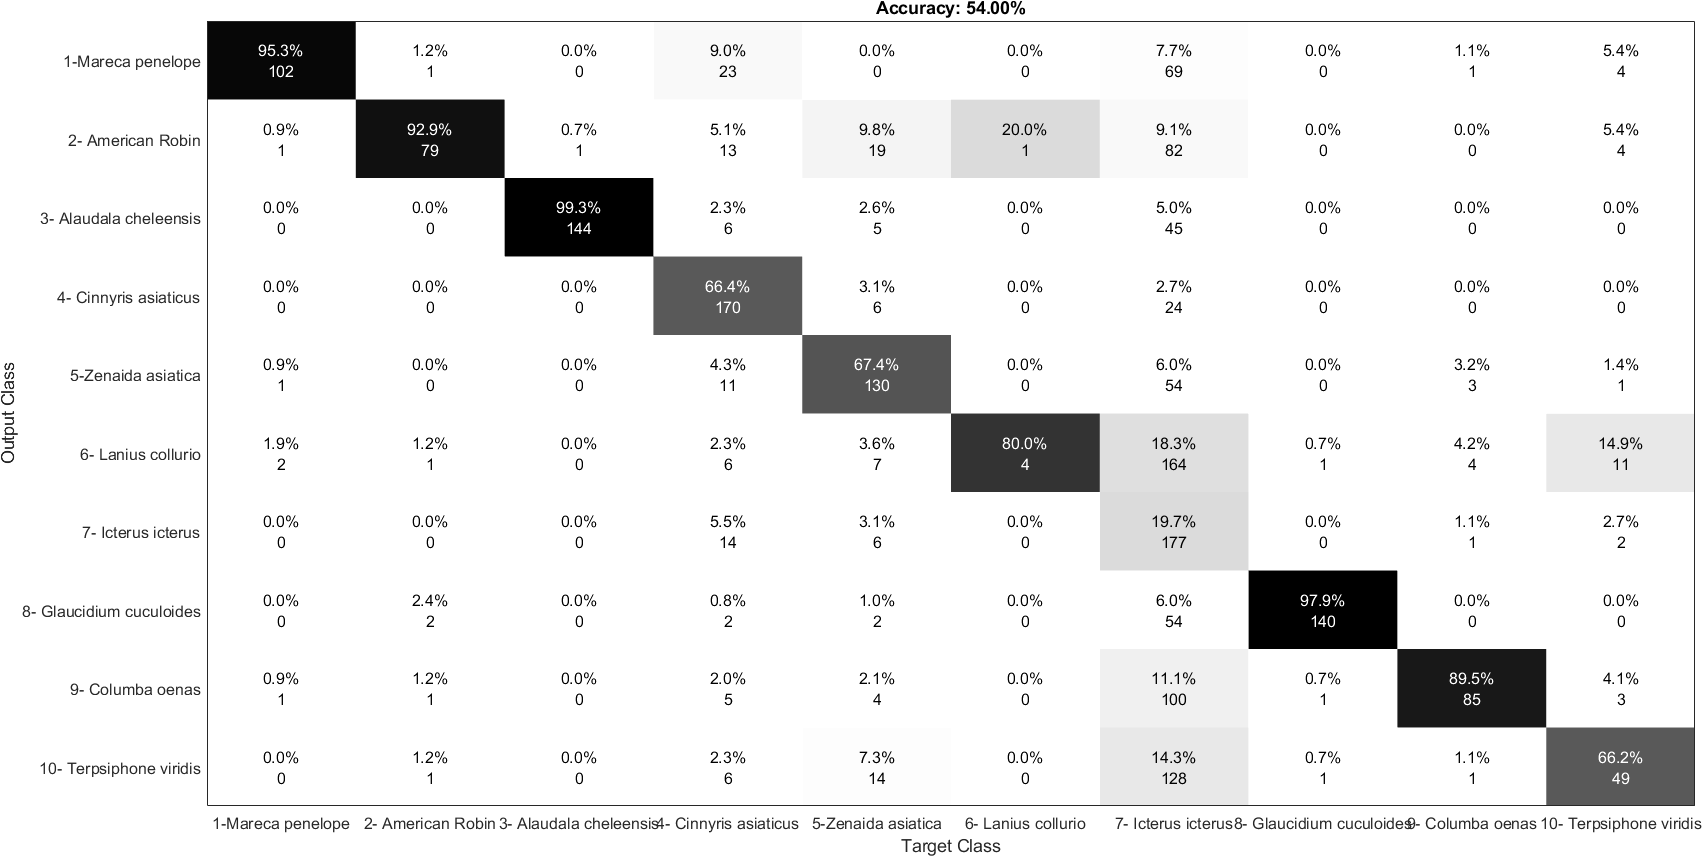
\includegraphics[width=\textwidth]{aymen-mfcc}
    \caption{MFCC confusion matrix.}
    \label{aymen-stft}
\end{figure}


In this section, we propose a comprehensive qualitative evaluation of the proposed algorithms. Two platforms are targets:
\begin{itemize}
\item AMD FX-8350 at 4 GHz having eight cores, 8 MB cache and 32 GB DRAM supported by NVIDIA GTX 1080 Ti with 11 GB RAM
\item Raspberry Pi 3 containing quad-core ARM Cortex-A53 running at 1.20 GHz with 1 GB of RAM.
\end{itemize}

\noindent The reason for choosing different platforms is that the lightweight algorithms can differ in implementations depending on the use-case and deployment strategy


